\documentclass[10pt]{article}
\usepackage[margin=0.56in]{geometry}
\usepackage{amsmath,amssymb,booktabs,graphicx,microtype,xcolor}

\usepackage[hidelinks]{hyperref}
\setlength{\parindent}{0pt}
\setlength{\parskip}{3pt}
\setlength{\abovedisplayskip}{3pt}
\setlength{\belowdisplayskip}{3pt}
\setlength{\textfloatsep}{5pt}
\renewcommand{\arraystretch}{1.08}

\title{\vspace{-1.15cm}\textbf{Two-Block $4{+}4{\to}8$ Circuit Formation with a $\mu$P Readout:\\Stationary Theory versus Training}}
\author{}
\date{\vspace{-1.3cm}}

\begin{document}
\maketitle
\vspace{-0.75cm}

\textbf{Result in one sentence.}
With the $\mu$P-like readout, parent-warm training forms the $4{+}4{\to}8$ circuit in 30 of the
theory's 34 $H_C$ cells with near-predicted shares; joint training composes only at
$\lambda_0=0.03$, and no cell has converged by 250k steps.

\textbf{Experiment.}
The $d4/d8$ setting of the theory (exact eight-bit cube; parents $\chi_L=x_1x_2x_3x_4$,
$\chi_R=x_5x_6x_7x_8$; target $\chi_8=\chi_L\chi_R$; $\gamma_4=\gamma_8=2$) in the bias-free
two-block residual ReLU network ($N=1024$, float64; both readouts read $h_2$), with
$\lambda_E=\lambda_2=\lambda_p=\lambda_8=\lambda_0$, $\lambda_1=(\lambda_1/\lambda_2)\lambda_0$
on a $9\times8$ grid, seed 0, both protocols; SGD with momentum 0.9, no noise, exactly 250k steps.
As in the $d2/d4$ runs the readouts have variance $1/N^2$ and rate $\eta/N$ ($\mu$P-like);
$V_1,V_2$ have variance $1/N$ and $E$ variance $1/d$, both at $\eta=10^{-3}$.  Parent-warm cells
start from $E$, $V_1$, $W_{d4}$ fitted to the parents read from $h_1$ (50k steps, same
optimizer; $R_4=0.366$).  The previous version of this report used the fan-in readout (variance
$1/N$, rate $\eta$; now in \texttt{fan\_in\_readout/}); the table repeats its values.

\textbf{Measurements.}  As in the Langevin report, with $\chi_L,\chi_R$ as parents and $\chi_8$ as
target: phases, $f_C$, $R_4=Q_4/Q_1^{(1)}$ (gate $5/32$) and the block-2 $4{+}4{\to}8$ shares
$\varphi_{\rm out}$, $\varphi_{\rm sq}$, $f_C^{\rm sq}$.  Fig.~4 adds the block-2 share of the parent
amplitude, what block 2's $d8$ producers read ($|w_{8,n}a_n|$-weighted pre-activation power on
the parents, on the $\chi_8$ mode made in block 1, a relay of route $D_1$, or on the singletons,
$D_2$), and $J/\min(F_C,F_D,F_0)$, the objective over the theory's minimal free energy
($F_0=3$).

\begin{center}
\small\setlength{\tabcolsep}{4pt}
\begin{tabular}{@{}lcccccc@{}}
\toprule
 & \multicolumn{2}{c}{Parent-warm} & \multicolumn{2}{c}{Joint} & \multicolumn{2}{c}{Lower objective} \\
Seed 0, $9\times8$ grid & $\mu$P & fan-in & $\mu$P & fan-in & $\mu$P & fan-in \\
\midrule
Phase agreement with theory & 77.8\% & 45.8\% & 54.2\% & 45.8\% & 75.0\% & 45.8\% \\
Gate $H_C\Leftrightarrow R_4>5/32$ (active cells) & 88.9\% & 73.1\% & 45.5\% & 76.9\% & 80.0\% & 76.9\% \\
Mean $|f_C-f_C^{\rm theory}|$ & 0.176 & 0.379 & 0.273 & 0.380 & 0.161 & 0.379 \\
Cells in $H_C$ (theory: 34) & 39 & 0 & 4 & 0 & 23 & 0 \\
\quad of which in the theory's $H_C$ region & 30 & 0 & 4 & 0 & 21 & 0 \\
Cells won (parent-warm / joint) & & & & & 26/46 & 43/29 \\
$R_4$ when the target is first fitted (median) & 0.36 & 0.093 & 0.23 & 0.067 & & \\
\midrule
Protocols select different phases & \multicolumn{6}{c}{40/72 cells ($\mu$P) versus 0/72 cells
(fan-in)} \\
\bottomrule
\end{tabular}
\end{center}

\textbf{Observations.}
(i) \emph{Parent-warm reproduces the compositional phase where it is predicted.}  In 30 of the
34 theory-$H_C$ cells it ends in $H_C$, with $f_C=0.60$--0.94 (theory 0.66--0.88; mean
$|\Delta f_C|=0.09$), $R_4=0.19$--0.44 (theory 0.18--0.41) and $\varphi_{\rm out}=0.77$--1.00,
rising with decay as for $d2/d4$ (mean 0.80 at $\lambda_0=10^{-4}$, $\ge0.92$ for
$\lambda_0\ge10^{-3}$).  Its block-2 $d8$ producers read the parents (median 98\%; relay, singletons
and degree-2 leakage $\le5\%$, $\le13\%$, $\le5\%$).  At $\lambda_0=10^{-4}$, $f_C$ rises with
$\lambda_1/\lambda_2$ (0.74 to 0.81) like the theory's (0.68 to 0.88); at
$\lambda_0=10^{-3}$--$10^{-2}$ it is 0.87--0.94 at every ratio, above the theory at small ratios.
(ii) \emph{Deviations sit at the edges.}  $H_C$ extends into the theory's $H_D$ region at weak
decay (9 cells, $\lambda_1/\lambda_2=10$--100, $\lambda_0\le3\times10^{-3}$, where the warm start's
block-1 parents have not yet decayed; $R_4<5/32$ in 5, the gate's only parent-warm failures).  At
strong decay the target is lost earlier than predicted: at $\lambda_0=0.1$ only
$\lambda_1/\lambda_2=0.1$ stays $H_C$ ($A_8=0.68$), $(0.1,0.3)$ keeps only the parents,
$(0.1,1$--$2)$ collapse, and $(0.03,5)$ ends at $A_8=0.49$, just below the labelling threshold.
(iii) \emph{Joint training composes only at $\lambda_0=0.03$} ($\lambda_1/\lambda_2=0.1$--2:
$f_C=0.67$--0.81 against 0.68--0.84, $\varphi_{\rm out}=0.86$--0.98) and collapses at
$\lambda_0\ge0.1$.  At $\lambda_0=10^{-3}$--$10^{-2}$ it fits the target in 4k--10k steps with
$R_4=0.19$--0.28, already above the gate, yet its block-2 $d8$ producers read mainly the $\chi_8$
mode built in block 1 (relay, median 58\%) and only 34\% the parents ($H_D$,
$f_C=0.15$--0.29); at $\lambda_0\le3\times10^{-4}$ they read mainly singletons (60\%).  The relay,
absent from the theory's two route families, rather than accessibility keeps joint training
direct; the protocols disagree in 40 of 72 cells, as for $d2/d4$.
(iv) \emph{Objectives barely separate the protocols.}  Where they disagree inside the theory's
$H_C$ region (25 cells) they differ by $\le4.1\%$; parent-warm's $H_C$ is lower in 16, joint's $H_D$
in 9 (five at $\lambda_0=10^{-4}$), so the lower-objective run is $H_C$ in 21 of the 34 cells.
(v) \emph{Nothing has converged.}  Every non-suppressed cell still loses 1.7--35\% of $J$ per 50k
steps.  $J$ is carried by the $E$, $V_1$, $V_2$ penalties while the readouts, trained at
$\eta/N\approx10^{-6}$, are still small ($\|w_8\|^2\le0.35$); at $\lambda_0\le3\times10^{-4}$ the
random initial hidden weights remain ($\|V\|^2\approx250$--1040).  In parent-warm $H_C$ cells
$J/F_C$ falls from 2.4--56 ($\lambda_0\le10^{-3}$) to 0.97--2.85 ($\lambda_0\ge3\times10^{-3}$;
1.05--1.13 at 0.03): $J$ approaches $F_C$ from above.
(vi) \emph{Why the readout matters.}  With the fan-in readout the target was fitted within 1k
steps at median $R_4=0.07$--0.09, and block 2 then relayed $D_1$; with the $\mu$P readout it takes
3k--156k steps and, after pretraining, is fitted through parents that are already accessible.  The
base-width run ($N_0=64$; separate figure) lies between them: target fitted in 1k--27k steps at median
$R_4=0.17$ (parent-warm) and 0.12 (joint), block 2 relaying $D_1$ (79--94\%), and $H_D$ in both
protocols except at $\lambda_0=0.1$ (3 and 2 $H_C$ cells).
(vii) Readout-free shares are higher ($f_C^{\rm sq}=0.69$--0.99 in parent-warm $H_C$ cells;
Fig.~2), so the readout favours the block-1 route; block 2 supplies 11--76\% of the parent
amplitude there, as each $4{+}4{\to}8$ unit also emits the parents,
$\sigma(a\chi_L+a\chi_R)=\tfrac a2(1+\chi_L+\chi_R+\chi_L\chi_R)$.  Final MSE is set by $\lambda_0$,
equally for both protocols (Fig.~3).

\textbf{Limits.}  One seed; no cell is stationary, so longer training or the $d2/d4$ rate
$10^{-2}$ is the next test of the weak-decay $H_C$ cells and the $f_C$ excess.

\begin{figure}[p]
\centering
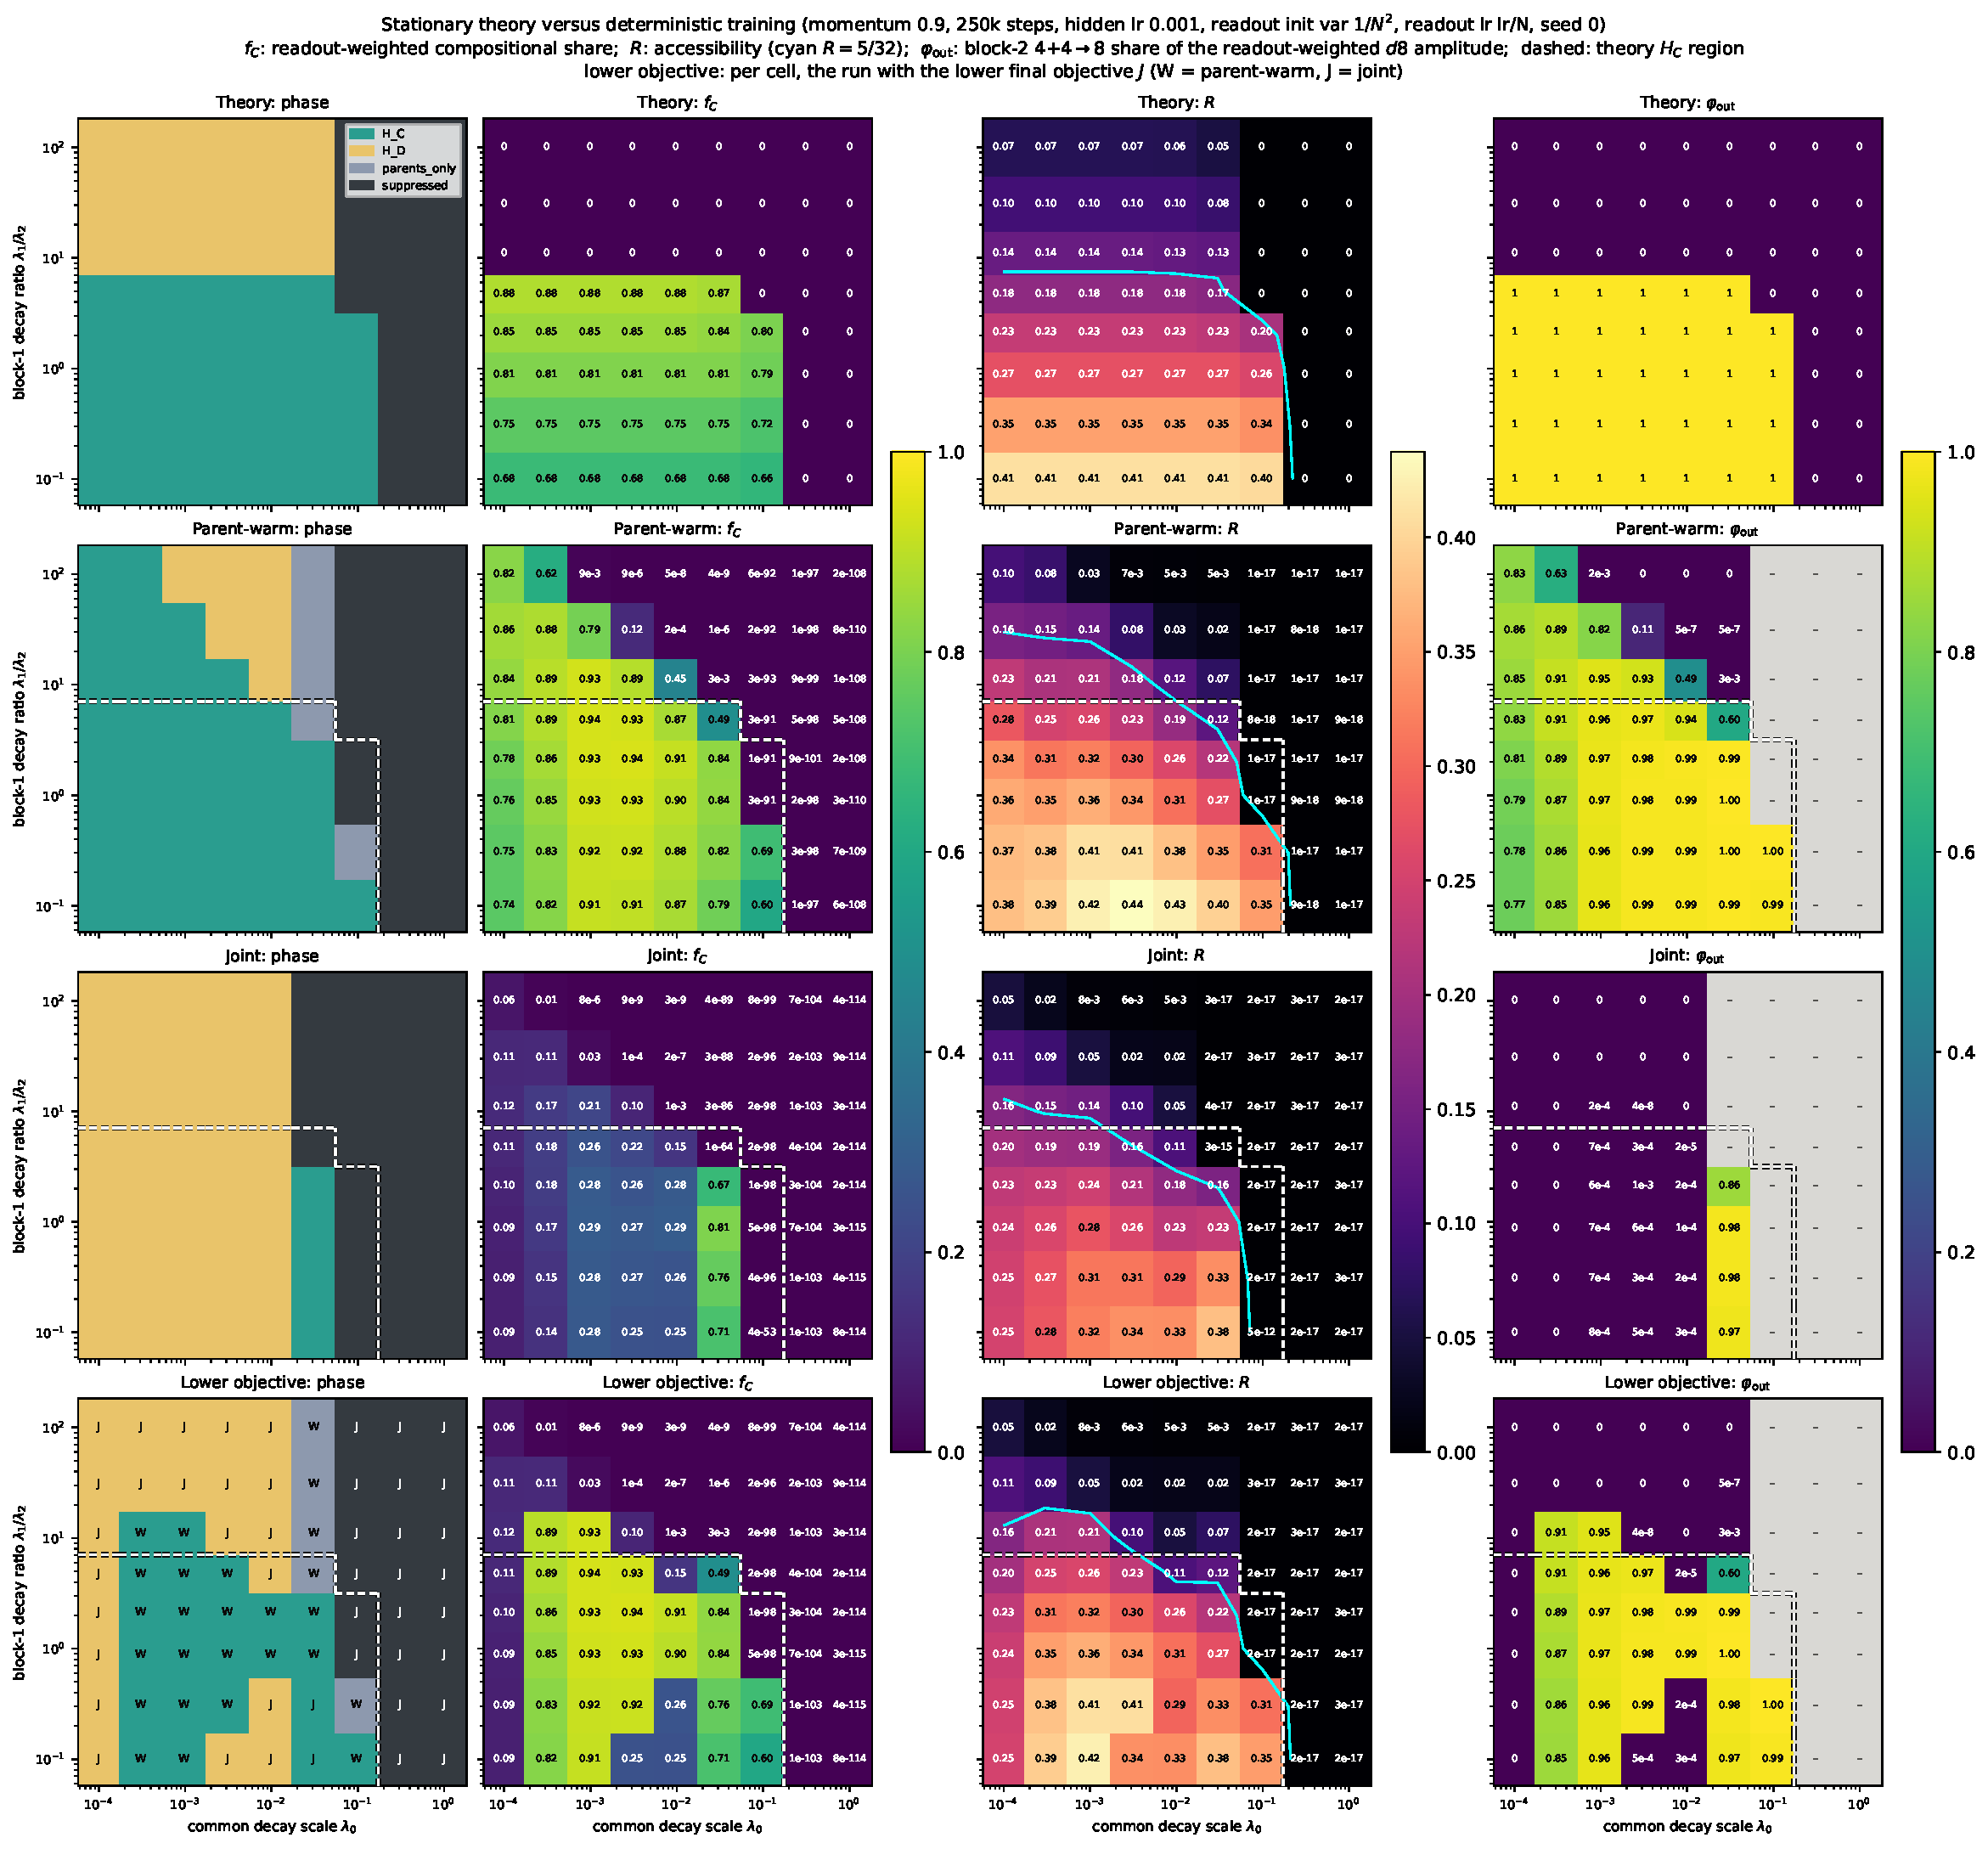
\includegraphics[width=\textwidth]{fig1_theory_vs_annealed.pdf}
\caption{\textbf{Theory, parent-warm, joint, and the lower-objective run per cell (rows, top to
bottom).}  In the bottom row each cell shows whichever of the two runs ended with the lower final
objective $J$ (W = parent-warm, J = joint).  Columns: phase, readout-weighted compositional share
$f_C$, accessibility $R_4$ (cyan: $R_4=5/32$), and the block-2 $4{+}4{\to}8$ share
$\varphi_{\rm out}$ of the readout-weighted $d8$ amplitude.  Dashed: theory $H_C$ region.  Grey:
no target mode produced.}
\end{figure}

\begin{figure}[p]
\centering
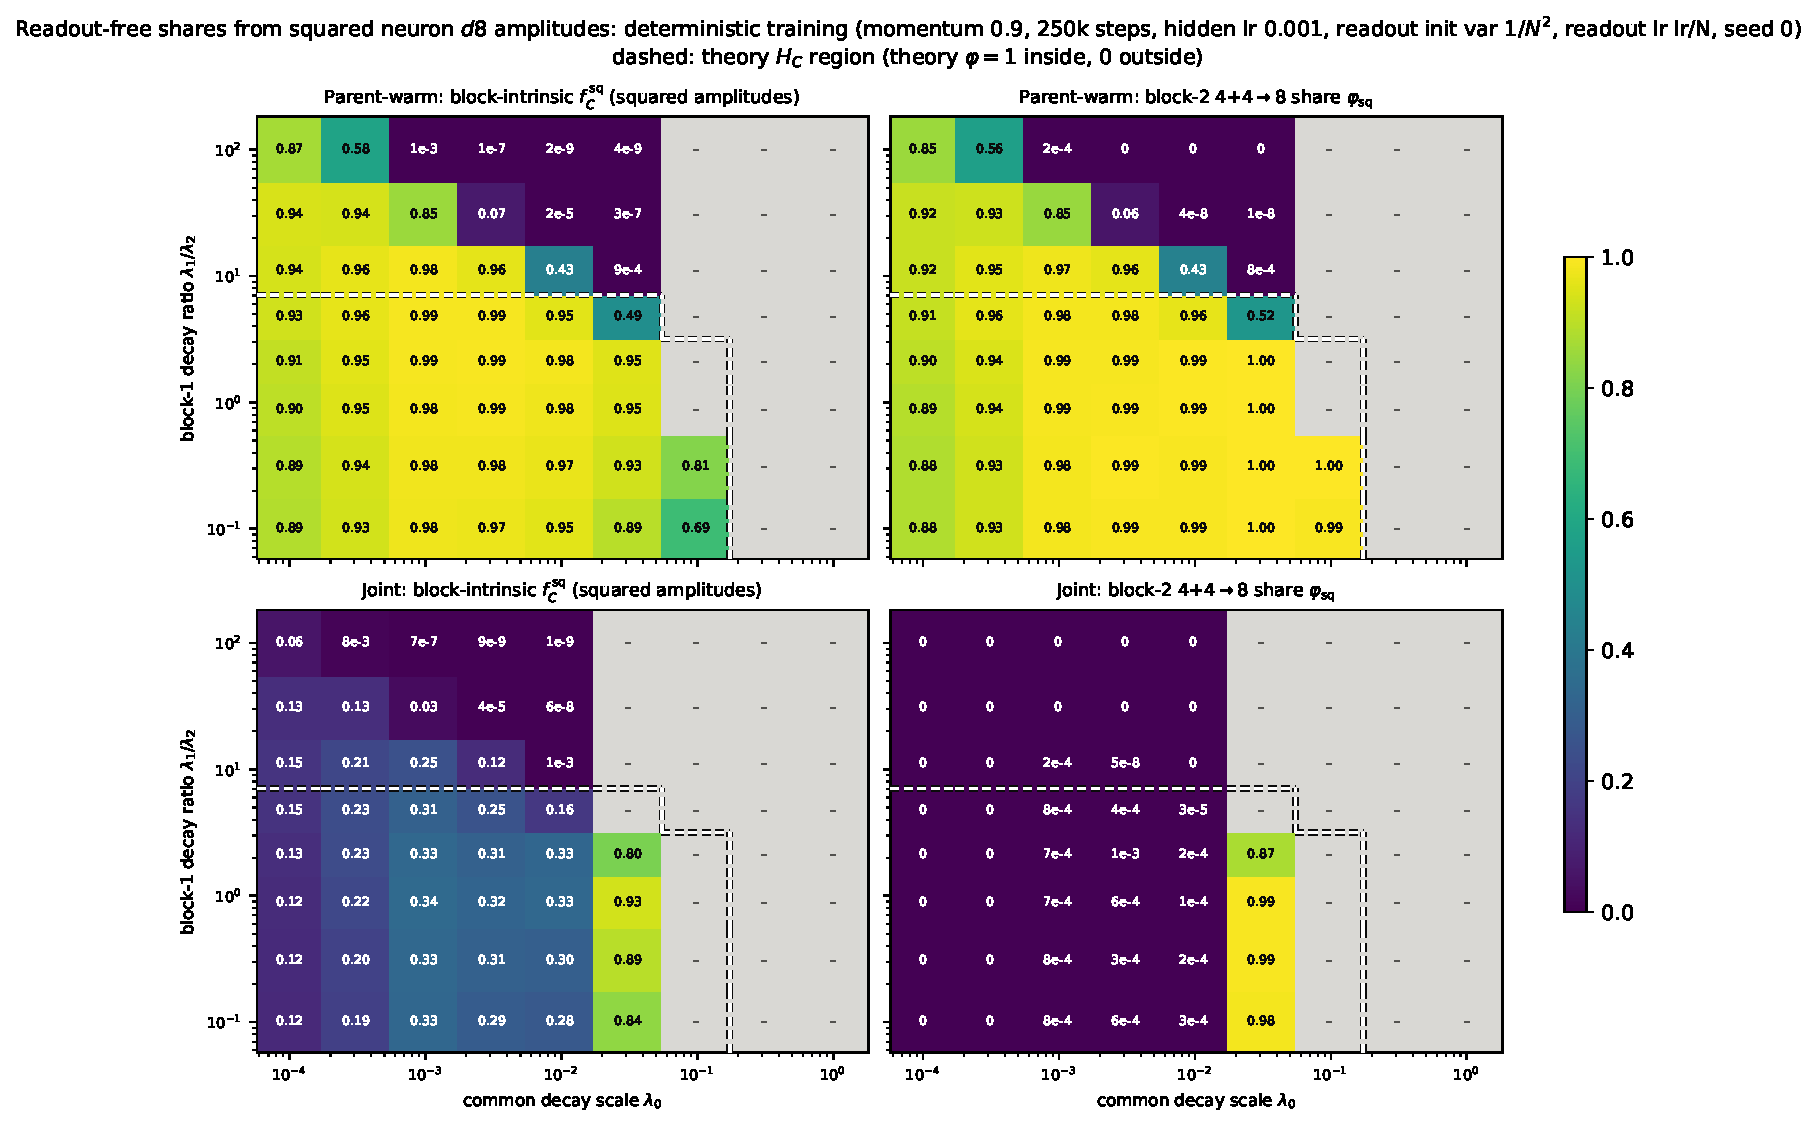
\includegraphics[width=0.78\textwidth]{fig2_block_intrinsic_shares.pdf}
\caption{\textbf{Readout-free shares} from squared neuron $d8$ amplitudes: $f_C^{\rm sq}$ (left)
and $\varphi_{\rm sq}$ (right); compare with columns 2 and 4 of Fig.~1.}
\vspace{6pt}
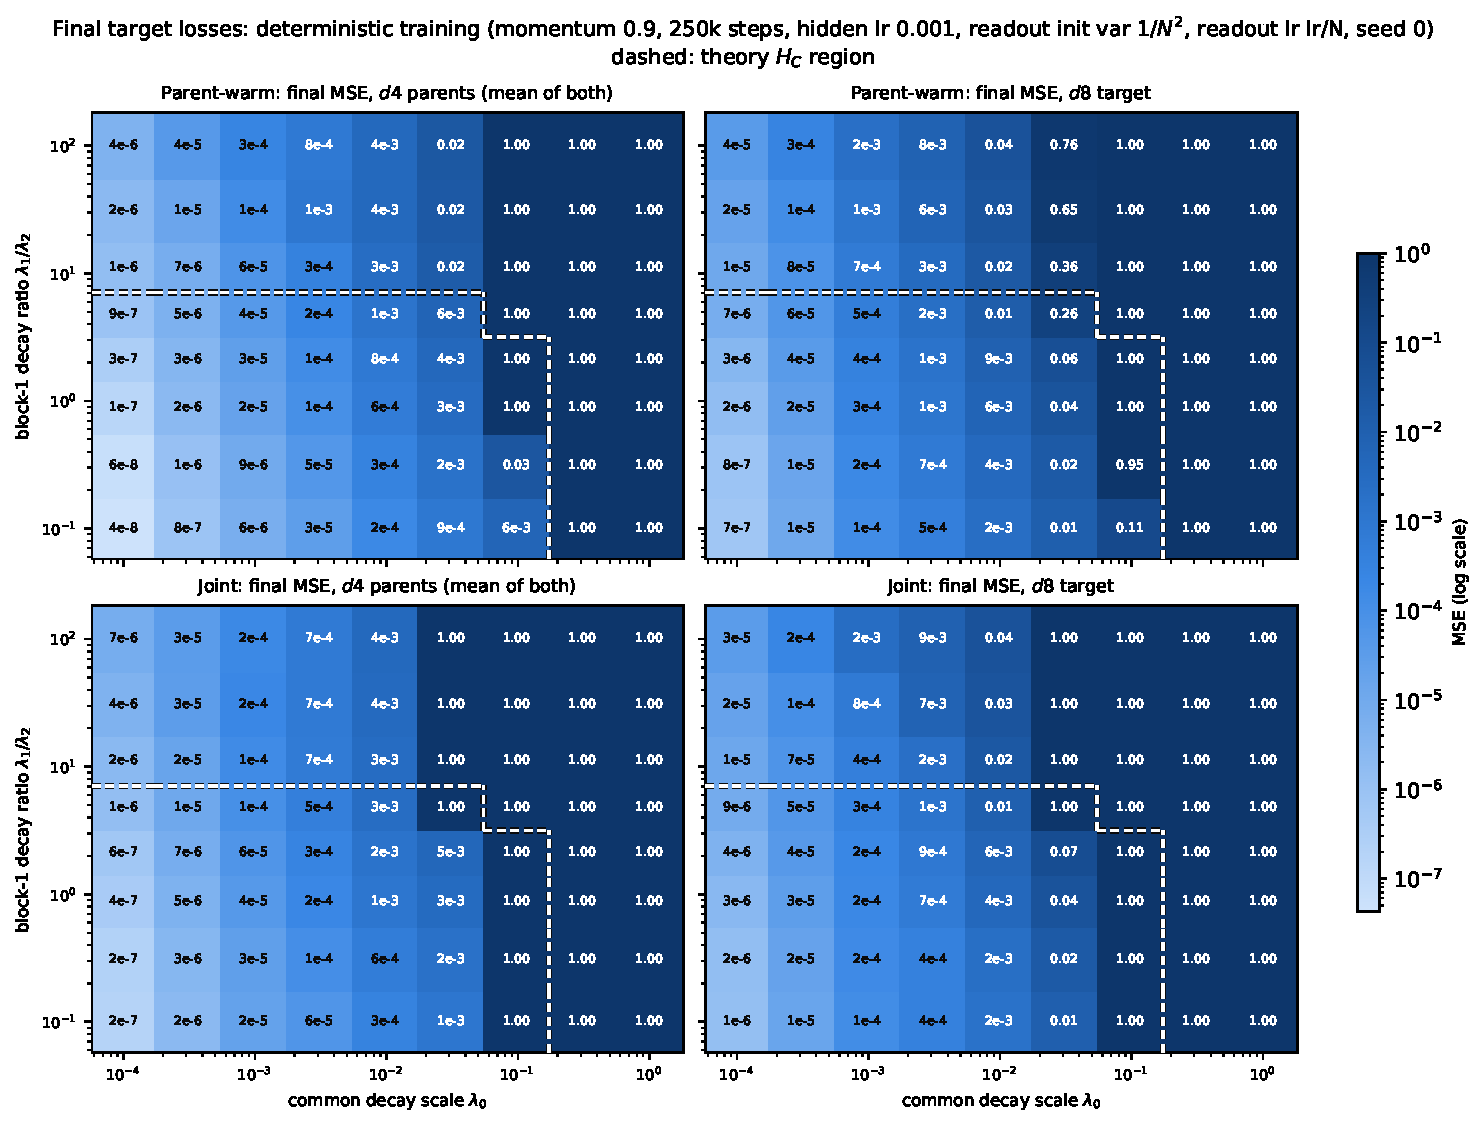
\includegraphics[width=0.78\textwidth]{fig3_final_mse.pdf}
\caption{\textbf{Final losses:} MSE of the two $d4$ parents (mean) and of the $d8$ target, log
scale.}
\end{figure}

\begin{figure}[p]
\centering
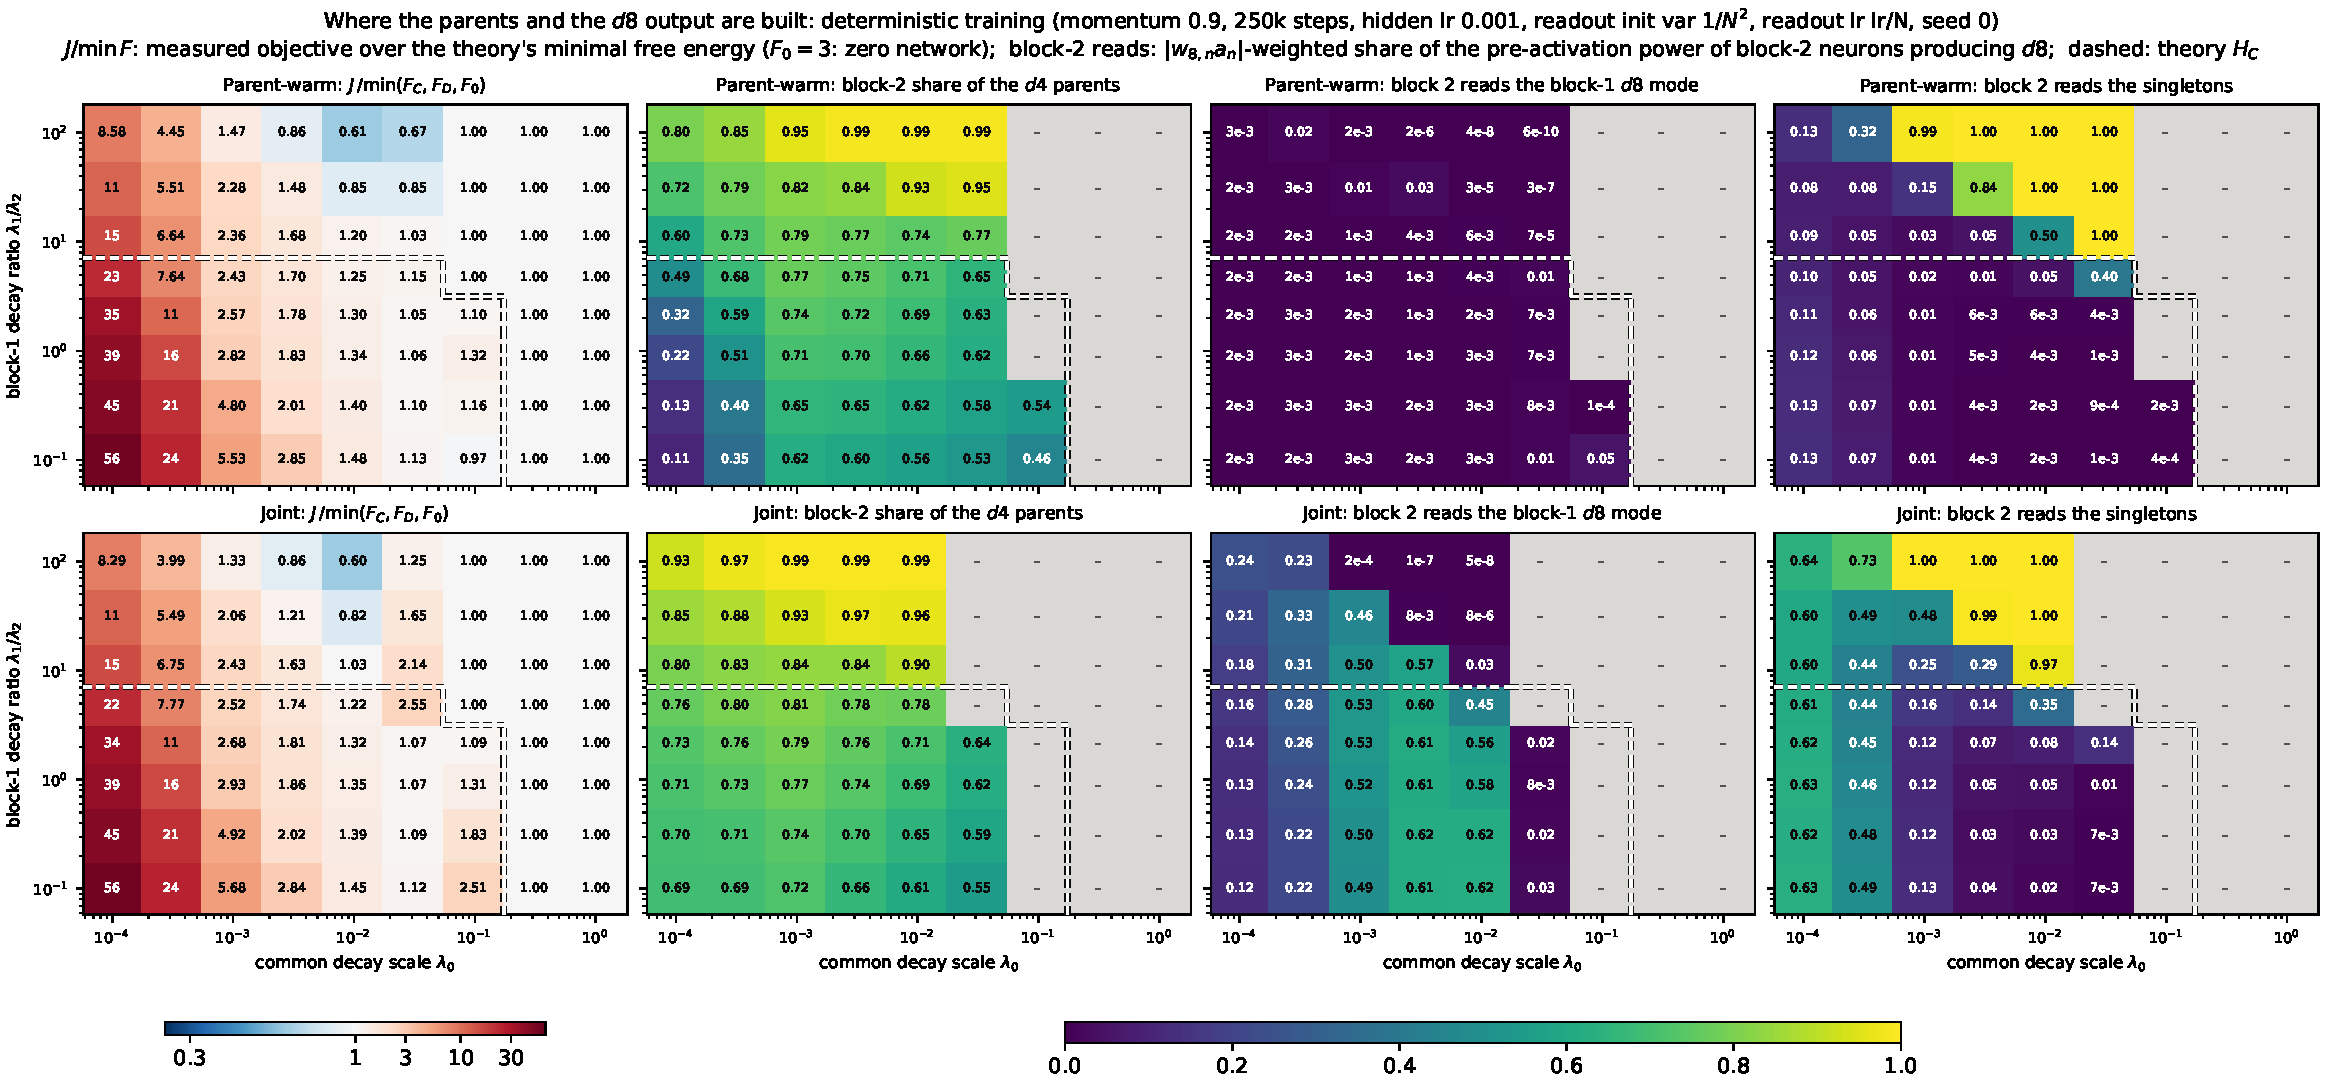
\includegraphics[width=\textwidth]{fig4_route_diagnostics.pdf}
\caption{\textbf{Where the parents and the $d8$ output are built} (rows: parent-warm, joint).
Columns: final objective over the theory's minimal free energy (blue: below it; red: above it);
block-2 share of the readout-weighted parent amplitude; share of the pre-activation power of
block-2 $d8$ producers (weighted by $|w_{8,n}a_n|$) on the $\chi_8$ mode built in block 1 (relay
of $D_1$) and on the eight singletons (direct $D_2$); the remainder is mostly the parents
($4{+}4{\to}8$).  Grey: block 2 produces no $d8$.}
\end{figure}

\end{document}
